% Options for packages loaded elsewhere
\PassOptionsToPackage{unicode}{hyperref}
\PassOptionsToPackage{hyphens}{url}
%
\documentclass[
]{article}
\usepackage{amsmath,amssymb}
\usepackage{iftex}
\ifPDFTeX
  \usepackage[T1]{fontenc}
  \usepackage[utf8]{inputenc}
  \usepackage{textcomp} % provide euro and other symbols
\else % if luatex or xetex
  \usepackage{unicode-math} % this also loads fontspec
  \defaultfontfeatures{Scale=MatchLowercase}
  \defaultfontfeatures[\rmfamily]{Ligatures=TeX,Scale=1}
\fi
\usepackage{lmodern}
\ifPDFTeX\else
  % xetex/luatex font selection
\fi
% Use upquote if available, for straight quotes in verbatim environments
\IfFileExists{upquote.sty}{\usepackage{upquote}}{}
\IfFileExists{microtype.sty}{% use microtype if available
  \usepackage[]{microtype}
  \UseMicrotypeSet[protrusion]{basicmath} % disable protrusion for tt fonts
}{}
\makeatletter
\@ifundefined{KOMAClassName}{% if non-KOMA class
  \IfFileExists{parskip.sty}{%
    \usepackage{parskip}
  }{% else
    \setlength{\parindent}{0pt}
    \setlength{\parskip}{6pt plus 2pt minus 1pt}}
}{% if KOMA class
  \KOMAoptions{parskip=half}}
\makeatother
\usepackage{xcolor}
\usepackage[margin=1in]{geometry}
\usepackage{color}
\usepackage{fancyvrb}
\newcommand{\VerbBar}{|}
\newcommand{\VERB}{\Verb[commandchars=\\\{\}]}
\DefineVerbatimEnvironment{Highlighting}{Verbatim}{commandchars=\\\{\}}
% Add ',fontsize=\small' for more characters per line
\usepackage{framed}
\definecolor{shadecolor}{RGB}{248,248,248}
\newenvironment{Shaded}{\begin{snugshade}}{\end{snugshade}}
\newcommand{\AlertTok}[1]{\textcolor[rgb]{0.94,0.16,0.16}{#1}}
\newcommand{\AnnotationTok}[1]{\textcolor[rgb]{0.56,0.35,0.01}{\textbf{\textit{#1}}}}
\newcommand{\AttributeTok}[1]{\textcolor[rgb]{0.13,0.29,0.53}{#1}}
\newcommand{\BaseNTok}[1]{\textcolor[rgb]{0.00,0.00,0.81}{#1}}
\newcommand{\BuiltInTok}[1]{#1}
\newcommand{\CharTok}[1]{\textcolor[rgb]{0.31,0.60,0.02}{#1}}
\newcommand{\CommentTok}[1]{\textcolor[rgb]{0.56,0.35,0.01}{\textit{#1}}}
\newcommand{\CommentVarTok}[1]{\textcolor[rgb]{0.56,0.35,0.01}{\textbf{\textit{#1}}}}
\newcommand{\ConstantTok}[1]{\textcolor[rgb]{0.56,0.35,0.01}{#1}}
\newcommand{\ControlFlowTok}[1]{\textcolor[rgb]{0.13,0.29,0.53}{\textbf{#1}}}
\newcommand{\DataTypeTok}[1]{\textcolor[rgb]{0.13,0.29,0.53}{#1}}
\newcommand{\DecValTok}[1]{\textcolor[rgb]{0.00,0.00,0.81}{#1}}
\newcommand{\DocumentationTok}[1]{\textcolor[rgb]{0.56,0.35,0.01}{\textbf{\textit{#1}}}}
\newcommand{\ErrorTok}[1]{\textcolor[rgb]{0.64,0.00,0.00}{\textbf{#1}}}
\newcommand{\ExtensionTok}[1]{#1}
\newcommand{\FloatTok}[1]{\textcolor[rgb]{0.00,0.00,0.81}{#1}}
\newcommand{\FunctionTok}[1]{\textcolor[rgb]{0.13,0.29,0.53}{\textbf{#1}}}
\newcommand{\ImportTok}[1]{#1}
\newcommand{\InformationTok}[1]{\textcolor[rgb]{0.56,0.35,0.01}{\textbf{\textit{#1}}}}
\newcommand{\KeywordTok}[1]{\textcolor[rgb]{0.13,0.29,0.53}{\textbf{#1}}}
\newcommand{\NormalTok}[1]{#1}
\newcommand{\OperatorTok}[1]{\textcolor[rgb]{0.81,0.36,0.00}{\textbf{#1}}}
\newcommand{\OtherTok}[1]{\textcolor[rgb]{0.56,0.35,0.01}{#1}}
\newcommand{\PreprocessorTok}[1]{\textcolor[rgb]{0.56,0.35,0.01}{\textit{#1}}}
\newcommand{\RegionMarkerTok}[1]{#1}
\newcommand{\SpecialCharTok}[1]{\textcolor[rgb]{0.81,0.36,0.00}{\textbf{#1}}}
\newcommand{\SpecialStringTok}[1]{\textcolor[rgb]{0.31,0.60,0.02}{#1}}
\newcommand{\StringTok}[1]{\textcolor[rgb]{0.31,0.60,0.02}{#1}}
\newcommand{\VariableTok}[1]{\textcolor[rgb]{0.00,0.00,0.00}{#1}}
\newcommand{\VerbatimStringTok}[1]{\textcolor[rgb]{0.31,0.60,0.02}{#1}}
\newcommand{\WarningTok}[1]{\textcolor[rgb]{0.56,0.35,0.01}{\textbf{\textit{#1}}}}
\usepackage{graphicx}
\makeatletter
\def\maxwidth{\ifdim\Gin@nat@width>\linewidth\linewidth\else\Gin@nat@width\fi}
\def\maxheight{\ifdim\Gin@nat@height>\textheight\textheight\else\Gin@nat@height\fi}
\makeatother
% Scale images if necessary, so that they will not overflow the page
% margins by default, and it is still possible to overwrite the defaults
% using explicit options in \includegraphics[width, height, ...]{}
\setkeys{Gin}{width=\maxwidth,height=\maxheight,keepaspectratio}
% Set default figure placement to htbp
\makeatletter
\def\fps@figure{htbp}
\makeatother
\setlength{\emergencystretch}{3em} % prevent overfull lines
\providecommand{\tightlist}{%
  \setlength{\itemsep}{0pt}\setlength{\parskip}{0pt}}
\setcounter{secnumdepth}{-\maxdimen} % remove section numbering
\usepackage{hyperref}
\usepackage{amsmath}
\usepackage{amssymb}
\usepackage{graphicx}
\usepackage{fontspec}
\setmainfont{Cambria}
\setsansfont{Franklin Gothic Demi Cond}
\setmonofont{Courier New}
\usepackage[margin=1in]{geometry}
\usepackage{titlesec}
\titleformat{\section}{\Huge\bfseries\color{black}}{\thesection}{1em}{}
\titleformat{\subsection}{\huge\bfseries\color{black}}{\thesubsection}{1em}{}
\titleformat{\subsubsection}{\LARGE\bfseries\color{black}}{\thesubsubsection}{1em}{}
\usepackage{tocloft}
\renewcommand{\cftsecfont}{\small}
\renewcommand{\cftsubsecfont}{\footnotesize}
\renewcommand{\cftsecpagefont}{\small}
\renewcommand{\cftsubsecpagefont}{\footnotesize}
\renewcommand{\cftsecleader}{\cftdotfill{\cftdotsep}}
\ifLuaTeX
  \usepackage{selnolig}  % disable illegal ligatures
\fi
\IfFileExists{bookmark.sty}{\usepackage{bookmark}}{\usepackage{hyperref}}
\IfFileExists{xurl.sty}{\usepackage{xurl}}{} % add URL line breaks if available
\urlstyle{same}
\hypersetup{
  hidelinks,
  pdfcreator={LaTeX via pandoc}}

\author{}
\date{\vspace{-2.5em}}

\begin{document}

\begin{titlepage}
    \begin{center}
        \textbf{\LARGE RÉPUBLIQUE DU SÉNÉGAL}\\[0.1cm]
        
\includegraphics[width=3cm]{Logo1.jpg} \\[0.1cm]  % Insère le chemin de ton logo
        \textbf{\large Un Peuple - Un But - Une Foi}\\[0.2cm]
        
        \textbf{\LARGE Ministère de l'Économie, du Plan et de la Coopération}\\[0.1cm]
        
\includegraphics[width=4cm]{Logo2.png} \\[0.1cm] 
        
        \textbf{\large Agence Nationale de la Statistique et de la Démographie (ANSD)}\\[0.2cm]
        
        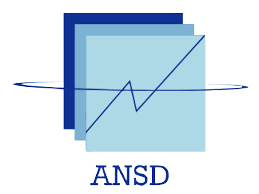
\includegraphics[width=4cm]{Logo3.png} \\[0.1cm]  
        
        \textbf{\large École nationale de la Statistique et de l'Analyse économique Pierre Ndiaye (ENSAE)}\\[0.4cm]
        
\includegraphics[width=3cm]{Logo4.png} \\[0.1cm]
        
        \textbf{\LARGE PROJET STATISTIQUES SOUS R }\\[0.3cm]
        \textbf{\Huge \color{black} \textsf{TP4 : Récupération des codes Admin 3 du Bénin et du Sénégal}}\\[0.2cm]
        \rule{\linewidth}{0.2mm} \\[0.5cm]
        
        \begin{minipage}{0.5\textwidth}
    \begin{flushleft} \large
        \emph{\textsf{Rédigé par :}}\\
        \textbf{Mame Balla BOUSSO}\\
        \textbf{Ameth FAYE}\\
        \textbf{EDIMA Biyenda Hildegarde}\\
        \textbf{Papa Amadou NIANG}\\
        \textit{Elèves ingénieurs statisticiens économistes}
    \end{flushleft}
\end{minipage}
        \hfill
        \begin{minipage}{0.4\textwidth}
            \begin{flushright} \large
                \emph{\textsf{Sous la supervision de :}} \\
                \textbf{M. Aboubacar HEMA}\\
                \textit{ANALYSTE DE RECHERCHE CHEZ IFPRI }
            \end{flushright}
        \end{minipage}

        \vfill

        {\large \textsf{Année scolaire : 2024/2025}}\\[0.5cm]
        
    \end{center}
\end{titlepage}

\hypertarget{introduction}{%
\section{Introduction}\label{introduction}}

Ce document présente le processus de fusion des bases de données afin de
récupérer les codes admin 3 pour chaque commune enquêtée dans la base
EHCVM.\\
Nous travaillons sur deux pays : le \textbf{Bénin} et le
\textbf{Sénégal}.\\
L'approche utilisée pour le Bénin est basée sur un nettoyage simple et
une fusion directe, tandis que pour le Sénégal, nous proposons une
démarche interactive permettant d'associer les communes en comparant
leur similarité textuelle.

\hypertarget{librairies-utilisuxe9es}{%
\section{Librairies Utilisées}\label{librairies-utilisuxe9es}}

Nous utilisons les librairies suivantes :

\begin{itemize}
\tightlist
\item
  \textbf{dplyr} : pour la manipulation des données (filtrage,
  transformation, fusion, suppression des colonnes problématiques,
  etc.).
\item
  \textbf{sf} : pour la manipulation des données spatiales (lecture des
  shapefiles, analyses géographiques).
\item
  \textbf{readxl} : pour la lecture des fichiers Excel.
\item
  \textbf{haven} : pour la lecture et l'écriture des fichiers de données
  au format Stata (.dta).
\item
  \textbf{labelled} : pour convertir les variables possédant des labels
  en facteurs.
\item
  \textbf{fuzzyjoin} : pour réaliser une jointure floue basée sur la
  distance de Levenshtein, permettant d'harmoniser les noms de communes
  malgré d'éventuelles différences typographiques.
\end{itemize}

\begin{Shaded}
\begin{Highlighting}[]
\FunctionTok{library}\NormalTok{(dplyr)}
\FunctionTok{library}\NormalTok{(stringi)}
\FunctionTok{library}\NormalTok{(stringr)}
\FunctionTok{library}\NormalTok{(fuzzyjoin)}
\FunctionTok{library}\NormalTok{(sf)}
\FunctionTok{library}\NormalTok{(haven)}
\FunctionTok{library}\NormalTok{(labelled)}
\FunctionTok{library}\NormalTok{(readxl)}
\end{Highlighting}
\end{Shaded}

\hypertarget{i-le-buxe9nin}{%
\section{I : Le Bénin}\label{i-le-buxe9nin}}

\hypertarget{pruxe9sentation-du-processus-pour-le-buxe9nin}{%
\subsection{Présentation du processus pour le
Bénin}\label{pruxe9sentation-du-processus-pour-le-buxe9nin}}

Pour le Bénin, nous disposons de trois sources de données :\\
1. \textbf{Shapefile} : Contient les limites administratives
(communes).\\
2. \textbf{Fichier Excel} : Renferme des informations complémentaires,
notamment les codes admin.\\
3. \textbf{Base EHCVM (Stata)} : Contient les données des enquêtes
individuelles.

\textbf{Objectif} : Fusionner ces sources pour associer, à chaque
commune de la base EHCVM, le code admin extrait des données
géographiques. Pour pallier les éventuelles différences d'orthographes
(erreurs typographiques, accents\ldots), nous utilisons une jointure
floue basée sur la distance de Levenshtein.

\hypertarget{uxe9tape-1-chargement-et-pruxe9paration-des-donnuxe9es}{%
\subsection{Étape 1 : Chargement et préparation des
données}\label{uxe9tape-1-chargement-et-pruxe9paration-des-donnuxe9es}}

Nous commençons par charger l'ensemble des données. La conversion des
variables labellisées en facteurs facilite par la suite le merge.

\begin{Shaded}
\begin{Highlighting}[]
\CommentTok{\# Chargement des données du Bénin}

\CommentTok{\# Shapefile des communes}
\NormalTok{data\_BEN }\OtherTok{\textless{}{-}} \FunctionTok{st\_read}\NormalTok{(}\StringTok{"data/Benin/shapefiles/geoBoundaries{-}BEN{-}ADM2.shp"}\NormalTok{)}
\end{Highlighting}
\end{Shaded}

\begin{verbatim}
## Reading layer `geoBoundaries-BEN-ADM2' from data source 
##   `D:\Projet statistique sous R\Projet-statistique-sous-R\TP 4\TP_Commune_Groupe2--ISEP3\data\Benin\shapefiles\geoBoundaries-BEN-ADM2.shp' 
##   using driver `ESRI Shapefile'
## Simple feature collection with 77 features and 5 fields
## Geometry type: POLYGON
## Dimension:     XY
## Bounding box:  xmin: 0.774575 ymin: 6.225748 xmax: 3.851701 ymax: 12.40861
## Geodetic CRS:  WGS 84
\end{verbatim}

\begin{Shaded}
\begin{Highlighting}[]
\CommentTok{\# Fichier Excel avec les codes admin}
\NormalTok{data\_BEN\_Pcode }\OtherTok{\textless{}{-}} \FunctionTok{read\_excel}\NormalTok{(}\StringTok{"data/Benin/shapefiles/ben\_adminboundaries\_tabulardata.xlsx"}\NormalTok{, }
                             \AttributeTok{sheet =} \StringTok{"ADM2"}\NormalTok{)}

\CommentTok{\# Base EHCVM (format Stata)}
\NormalTok{data }\OtherTok{\textless{}{-}} \FunctionTok{read\_dta}\NormalTok{(}\StringTok{"data/Benin/ehcvm/ehcvm\_individu\_ben2021.dta"}\NormalTok{)}

\CommentTok{\# Conversion des variables labellisées en facteurs}
\NormalTok{data }\OtherTok{\textless{}{-}} \FunctionTok{to\_factor}\NormalTok{(data)}
\end{Highlighting}
\end{Shaded}

\hypertarget{uxe9tape-2-nettoyage-des-noms-de-communes}{%
\subsection{Étape 2 : Nettoyage des noms de
communes}\label{uxe9tape-2-nettoyage-des-noms-de-communes}}

Afin d'assurer une correspondance correcte entre les bases, nous
normalisons les noms en : - Remplaçant les caractères accentués (É, È,
é, è) par leur équivalent non accentué. - Convertissant tous les noms en
minuscules.

\begin{Shaded}
\begin{Highlighting}[]
\CommentTok{\# Nettoyage pour la base EHCVM}
\NormalTok{data}\SpecialCharTok{$}\NormalTok{commune }\OtherTok{\textless{}{-}} \FunctionTok{gsub}\NormalTok{(}\StringTok{"[ÉÈéè]"}\NormalTok{, }\StringTok{"e"}\NormalTok{, data}\SpecialCharTok{$}\NormalTok{commune)}
\NormalTok{data }\OtherTok{\textless{}{-}}\NormalTok{ data }\SpecialCharTok{\%\textgreater{}\%} \FunctionTok{mutate}\NormalTok{(}\AttributeTok{commune =} \FunctionTok{tolower}\NormalTok{(commune))}

\CommentTok{\# Nettoyage pour le shapefile et le fichier Excel}
\NormalTok{data\_BEN }\OtherTok{\textless{}{-}}\NormalTok{ data\_BEN }\SpecialCharTok{\%\textgreater{}\%} \FunctionTok{mutate}\NormalTok{(}\AttributeTok{shapeName =} \FunctionTok{tolower}\NormalTok{(shapeName))}
\NormalTok{data\_BEN\_Pcode }\OtherTok{\textless{}{-}}\NormalTok{ data\_BEN\_Pcode }\SpecialCharTok{\%\textgreater{}\%} \FunctionTok{mutate}\NormalTok{(}\AttributeTok{ADM2\_FR =} \FunctionTok{tolower}\NormalTok{(ADM2\_FR))}
\end{Highlighting}
\end{Shaded}

\hypertarget{uxe9tape-3-fusion-des-donnuxe9es-guxe9ographiques}{%
\subsection{Étape 3 : Fusion des données
géographiques}\label{uxe9tape-3-fusion-des-donnuxe9es-guxe9ographiques}}

Nous fusionnons le shapefile avec le fichier Excel afin d'associer les
informations complémentaires (codes admin) aux limites administratives.

\begin{Shaded}
\begin{Highlighting}[]
\NormalTok{data\_BEN\_fin }\OtherTok{\textless{}{-}} \FunctionTok{merge}\NormalTok{(data\_BEN, data\_BEN\_Pcode, }\AttributeTok{by.x =} \StringTok{"shapeName"}\NormalTok{, }\AttributeTok{by.y =} \StringTok{"ADM2\_FR"}\NormalTok{)}
\end{Highlighting}
\end{Shaded}

\hypertarget{uxe9tape-4-fusion-finale-avec-la-base-ehcvm-via-une-jointure-floue}{%
\subsection{Étape 4 : Fusion finale avec la base EHCVM via une jointure
floue}\label{uxe9tape-4-fusion-finale-avec-la-base-ehcvm-via-une-jointure-floue}}

Afin de corriger les différences éventuelles d'orthographe entre les
noms de communes dans la base EHCVM et dans les données géographiques,
nous utilisons une jointure floue. La fonction
\texttt{stringdist\_left\_join} du package \textbf{fuzzyjoin} permet de
calculer la distance de Levenshtein entre les chaînes et de
sélectionner, pour chaque commune, le match présentant la distance
minimale.

\begin{Shaded}
\begin{Highlighting}[]
\NormalTok{data\_merge\_BEN }\OtherTok{\textless{}{-}} \FunctionTok{stringdist\_left\_join}\NormalTok{(}
\NormalTok{  data\_BEN\_fin, data, }
  \AttributeTok{by =} \FunctionTok{c}\NormalTok{(}\StringTok{"shapeName"} \OtherTok{=} \StringTok{"commune"}\NormalTok{), }
  \AttributeTok{method =} \StringTok{"lv"}\NormalTok{, }
  \AttributeTok{max\_dist =} \DecValTok{5}\NormalTok{,         }\CommentTok{\# Valeur ajustable selon la tolérance souhaitée}
  \AttributeTok{distance\_col =} \StringTok{"distance"}
\NormalTok{)}

\CommentTok{\# Pour chaque commune de la base EHCVM, ne conserver que la correspondance avec la distance minimale}
\NormalTok{data\_merge\_BEN }\OtherTok{\textless{}{-}}\NormalTok{ data\_merge\_BEN }\SpecialCharTok{\%\textgreater{}\%}
  \FunctionTok{group\_by}\NormalTok{(commune) }\SpecialCharTok{\%\textgreater{}\%}
  \FunctionTok{filter}\NormalTok{(distance }\SpecialCharTok{==} \FunctionTok{min}\NormalTok{(distance)) }\SpecialCharTok{\%\textgreater{}\%}
  \FunctionTok{ungroup}\NormalTok{()}
\end{Highlighting}
\end{Shaded}

\begin{quote}
\textbf{Remarque :} Par exemple, si la base EHCVM recense une commune
sous le nom « cotonou » alors que le shapefile la nomme « cotounou » (ou
une variante proche), la jointure floue permet d'identifier le meilleur
match en tenant compte de la distance de Levenshtein.
\end{quote}

\hypertarget{uxe9tape-5-pruxe9paration-de-la-base-finale-et-exportation}{%
\subsection{Étape 5 : Préparation de la base finale et
exportation}\label{uxe9tape-5-pruxe9paration-de-la-base-finale-et-exportation}}

La base fusionnée contient une variable \texttt{geometry} qui n'est pas
requise pour une utilisation ultérieure dans Stata ainsi que toute
variable de type \texttt{list}. Nous les retirons avant d'exporter la
base au format Stata.

\begin{Shaded}
\begin{Highlighting}[]
\CommentTok{\# Suppression de la variable geometry}
\NormalTok{data\_merge\_BEN }\OtherTok{\textless{}{-}} \FunctionTok{st\_drop\_geometry}\NormalTok{(data\_merge\_BEN)}
\NormalTok{data\_merge\_BEN }\OtherTok{\textless{}{-}}\NormalTok{ data\_merge\_BEN }\SpecialCharTok{\%\textgreater{}\%} \FunctionTok{select\_if}\NormalTok{(}\SpecialCharTok{\textasciitilde{}} \SpecialCharTok{!}\FunctionTok{is.list}\NormalTok{(.))}

\CommentTok{\# Exportation de la base finale au format Stata}
\FunctionTok{write\_dta}\NormalTok{(data\_merge\_BEN, }\StringTok{"Outputs/data\_final\_BEN.dta"}\NormalTok{)}
\end{Highlighting}
\end{Shaded}

\hypertarget{ii-le-suxe9nuxe9gal}{%
\section{II : Le Sénégal}\label{ii-le-suxe9nuxe9gal}}

\hypertarget{pruxe9sentation-du-processus-pour-le-suxe9nuxe9gal}{%
\subsection{Présentation du processus pour le
Sénégal}\label{pruxe9sentation-du-processus-pour-le-suxe9nuxe9gal}}

Pour le Sénégal, les noms de communes dans les différentes sources
peuvent présenter des variations (abréviations, accents, fautes
d'orthographe).\\
\textbf{Objectif} : Proposer une démarche interactive afin d'associer
chaque commune du shapefile à celle de la base EHCVM en s'appuyant sur
un score de similarité calculé sur la base de la distance de
Levenshtein.

\hypertarget{uxe9tape-1-duxe9finition-des-fonctions-de-nettoyage-et-de-similarituxe9}{%
\subsubsection{Étape 1 : Définition des fonctions de nettoyage et de
similarité}\label{uxe9tape-1-duxe9finition-des-fonctions-de-nettoyage-et-de-similarituxe9}}

\hypertarget{fonction-de-nettoyage-des-noms-de-communes}{%
\paragraph{1.1 Fonction de nettoyage des noms de
communes}\label{fonction-de-nettoyage-des-noms-de-communes}}

Cette fonction transforme les noms en minuscules, retire les préfixes
inutiles (par exemple «COM.»), enlève les accents et supprime les
espaces pour faciliter la comparaison.

\begin{Shaded}
\begin{Highlighting}[]
\NormalTok{nettoyage\_commune }\OtherTok{\textless{}{-}} \ControlFlowTok{function}\NormalTok{(x) \{}
\NormalTok{  x }\SpecialCharTok{\%\textgreater{}\%}
    \FunctionTok{tolower}\NormalTok{() }\SpecialCharTok{\%\textgreater{}\%}
    \FunctionTok{str\_replace\_all}\NormalTok{(}\StringTok{"\^{}(com}\SpecialCharTok{\textbackslash{}\textbackslash{}}\StringTok{.?}\SpecialCharTok{\textbackslash{}\textbackslash{}}\StringTok{s*|com}\SpecialCharTok{\textbackslash{}\textbackslash{}}\StringTok{s+|commune}\SpecialCharTok{\textbackslash{}\textbackslash{}}\StringTok{s*(de)?}\SpecialCharTok{\textbackslash{}\textbackslash{}}\StringTok{s*)"}\NormalTok{, }\StringTok{""}\NormalTok{) }\SpecialCharTok{\%\textgreater{}\%}
    \FunctionTok{stri\_trans\_general}\NormalTok{(}\StringTok{"Latin{-}ASCII"}\NormalTok{) }\SpecialCharTok{\%\textgreater{}\%}
    \FunctionTok{str\_replace\_all}\NormalTok{(}\StringTok{"[\textquotesingle{}’‘´\textasciigrave{}]"}\NormalTok{, }\StringTok{""}\NormalTok{) }\SpecialCharTok{\%\textgreater{}\%}
    \FunctionTok{str\_replace\_all}\NormalTok{(}\StringTok{"[\^{}[:alnum:] ]+"}\NormalTok{, }\StringTok{" "}\NormalTok{) }\SpecialCharTok{\%\textgreater{}\%}
    \FunctionTok{str\_squish}\NormalTok{() }\SpecialCharTok{\%\textgreater{}\%}
    \FunctionTok{str\_replace\_all}\NormalTok{(}\StringTok{" "}\NormalTok{, }\StringTok{""}\NormalTok{)}
\NormalTok{\}}

\CommentTok{\# Exemple d\textquotesingle{}utilisation}
\NormalTok{exemple\_commune }\OtherTok{\textless{}{-}} \StringTok{"COM. SénéGalKèmo"}
\FunctionTok{cat}\NormalTok{(}\StringTok{"Avant nettoyage : "}\NormalTok{, exemple\_commune, }\StringTok{"}\SpecialCharTok{\textbackslash{}n}\StringTok{"}\NormalTok{)}
\end{Highlighting}
\end{Shaded}

\begin{verbatim}
## Avant nettoyage :  COM. SénéGalKèmo
\end{verbatim}

\begin{Shaded}
\begin{Highlighting}[]
\FunctionTok{cat}\NormalTok{(}\StringTok{"Après nettoyage : "}\NormalTok{, }\FunctionTok{nettoyage\_commune}\NormalTok{(exemple\_commune), }\StringTok{"}\SpecialCharTok{\textbackslash{}n}\StringTok{"}\NormalTok{)}
\end{Highlighting}
\end{Shaded}

\begin{verbatim}
## Après nettoyage :  senegalkemo
\end{verbatim}

\hypertarget{fonction-de-calcul-de-la-distance-de-levenshtein}{%
\paragraph{1.2 Fonction de calcul de la distance de
Levenshtein}\label{fonction-de-calcul-de-la-distance-de-levenshtein}}

Cette fonction calcule la distance minimale (nombre d'opérations)
nécessaire pour transformer une chaîne en une autre.

\begin{Shaded}
\begin{Highlighting}[]
\NormalTok{levenshtein\_distance }\OtherTok{\textless{}{-}} \ControlFlowTok{function}\NormalTok{(s, t) \{}
\NormalTok{  s\_chars }\OtherTok{\textless{}{-}} \FunctionTok{unlist}\NormalTok{(}\FunctionTok{strsplit}\NormalTok{(s, }\AttributeTok{split =} \StringTok{""}\NormalTok{))}
\NormalTok{  t\_chars }\OtherTok{\textless{}{-}} \FunctionTok{unlist}\NormalTok{(}\FunctionTok{strsplit}\NormalTok{(t, }\AttributeTok{split =} \StringTok{""}\NormalTok{))}
\NormalTok{  m }\OtherTok{\textless{}{-}} \FunctionTok{length}\NormalTok{(s\_chars)}
\NormalTok{  n }\OtherTok{\textless{}{-}} \FunctionTok{length}\NormalTok{(t\_chars)}
\NormalTok{  d }\OtherTok{\textless{}{-}} \FunctionTok{matrix}\NormalTok{(}\DecValTok{0}\NormalTok{, }\AttributeTok{nrow =}\NormalTok{ m }\SpecialCharTok{+} \DecValTok{1}\NormalTok{, }\AttributeTok{ncol =}\NormalTok{ n }\SpecialCharTok{+} \DecValTok{1}\NormalTok{)}
  \ControlFlowTok{for}\NormalTok{(i }\ControlFlowTok{in} \DecValTok{1}\SpecialCharTok{:}\NormalTok{(m }\SpecialCharTok{+} \DecValTok{1}\NormalTok{)) \{ d[i, }\DecValTok{1}\NormalTok{] }\OtherTok{\textless{}{-}}\NormalTok{ i }\SpecialCharTok{{-}} \DecValTok{1}\NormalTok{ \}}
  \ControlFlowTok{for}\NormalTok{(j }\ControlFlowTok{in} \DecValTok{1}\SpecialCharTok{:}\NormalTok{(n }\SpecialCharTok{+} \DecValTok{1}\NormalTok{)) \{ d[}\DecValTok{1}\NormalTok{, j] }\OtherTok{\textless{}{-}}\NormalTok{ j }\SpecialCharTok{{-}} \DecValTok{1}\NormalTok{ \}}
  \ControlFlowTok{for}\NormalTok{(i }\ControlFlowTok{in} \DecValTok{1}\SpecialCharTok{:}\NormalTok{m) \{}
    \ControlFlowTok{for}\NormalTok{(j }\ControlFlowTok{in} \DecValTok{1}\SpecialCharTok{:}\NormalTok{n) \{}
\NormalTok{      cost }\OtherTok{\textless{}{-}} \FunctionTok{ifelse}\NormalTok{(s\_chars[i] }\SpecialCharTok{==}\NormalTok{ t\_chars[j], }\DecValTok{0}\NormalTok{, }\DecValTok{1}\NormalTok{)}
\NormalTok{      d[i }\SpecialCharTok{+} \DecValTok{1}\NormalTok{, j }\SpecialCharTok{+} \DecValTok{1}\NormalTok{] }\OtherTok{\textless{}{-}} \FunctionTok{min}\NormalTok{(d[i, j }\SpecialCharTok{+} \DecValTok{1}\NormalTok{] }\SpecialCharTok{+} \DecValTok{1}\NormalTok{,}
\NormalTok{                             d[i }\SpecialCharTok{+} \DecValTok{1}\NormalTok{, j] }\SpecialCharTok{+} \DecValTok{1}\NormalTok{,}
\NormalTok{                             d[i, j] }\SpecialCharTok{+}\NormalTok{ cost)}
\NormalTok{    \}}
\NormalTok{  \}}
  \FunctionTok{return}\NormalTok{(d[m }\SpecialCharTok{+} \DecValTok{1}\NormalTok{, n }\SpecialCharTok{+} \DecValTok{1}\NormalTok{])}
\NormalTok{\}}

\CommentTok{\# Exemple d\textquotesingle{}utilisation}
\NormalTok{s1 }\OtherTok{\textless{}{-}} \StringTok{"chat"}
\NormalTok{s2 }\OtherTok{\textless{}{-}} \StringTok{"chats"}
\FunctionTok{cat}\NormalTok{(}\StringTok{"Distance de Levenshtein entre \textquotesingle{}"}\NormalTok{, s1, }\StringTok{"\textquotesingle{} et \textquotesingle{}"}\NormalTok{, s2, }\StringTok{"\textquotesingle{} : "}\NormalTok{, }
    \FunctionTok{levenshtein\_distance}\NormalTok{(s1, s2), }\StringTok{"}\SpecialCharTok{\textbackslash{}n}\StringTok{"}\NormalTok{, }\AttributeTok{sep =} \StringTok{""}\NormalTok{)}
\end{Highlighting}
\end{Shaded}

\begin{verbatim}
## Distance de Levenshtein entre 'chat' et 'chats' : 1
\end{verbatim}

\hypertarget{fonction-de-calcul-de-la-similarituxe9-normalisuxe9e}{%
\paragraph{1.3 Fonction de calcul de la similarité
normalisée}\label{fonction-de-calcul-de-la-similarituxe9-normalisuxe9e}}

Cette fonction utilise la distance de Levenshtein pour calculer un score
de similarité entre 0 et 1.

\begin{Shaded}
\begin{Highlighting}[]
\NormalTok{similarity }\OtherTok{\textless{}{-}} \ControlFlowTok{function}\NormalTok{(s, t) \{}
\NormalTok{  d }\OtherTok{\textless{}{-}} \FunctionTok{levenshtein\_distance}\NormalTok{(s, t)}
\NormalTok{  max\_len }\OtherTok{\textless{}{-}} \FunctionTok{max}\NormalTok{(}\FunctionTok{nchar}\NormalTok{(s), }\FunctionTok{nchar}\NormalTok{(t))}
  \ControlFlowTok{if}\NormalTok{(max\_len }\SpecialCharTok{==} \DecValTok{0}\NormalTok{) }\FunctionTok{return}\NormalTok{(}\DecValTok{1}\NormalTok{)}
  \FunctionTok{return}\NormalTok{(}\DecValTok{1} \SpecialCharTok{{-}}\NormalTok{ d }\SpecialCharTok{/}\NormalTok{ max\_len)}
\NormalTok{\}}

\CommentTok{\# Exemple d\textquotesingle{}utilisation}
\FunctionTok{cat}\NormalTok{(}\StringTok{"Similarité entre \textquotesingle{}"}\NormalTok{, s1, }\StringTok{"\textquotesingle{} et \textquotesingle{}"}\NormalTok{, s2, }\StringTok{"\textquotesingle{} : "}\NormalTok{, }
    \FunctionTok{similarity}\NormalTok{(s1, s2), }\StringTok{"}\SpecialCharTok{\textbackslash{}n}\StringTok{"}\NormalTok{, }\AttributeTok{sep =} \StringTok{""}\NormalTok{)}
\end{Highlighting}
\end{Shaded}

\begin{verbatim}
## Similarité entre 'chat' et 'chats' : 0.8
\end{verbatim}

\hypertarget{fonction-pour-calculer-la-matrice-de-similarituxe9}{%
\paragraph{1.4 Fonction pour calculer la matrice de
similarité}\label{fonction-pour-calculer-la-matrice-de-similarituxe9}}

Cette fonction construit une matrice dans laquelle chaque case
correspond au score de similarité entre un nom issu du shapefile et un
nom de la base EHCVM.

\begin{Shaded}
\begin{Highlighting}[]
\NormalTok{compute\_similarity\_matrix }\OtherTok{\textless{}{-}} \ControlFlowTok{function}\NormalTok{(shape\_communes, ehcvm\_communes, }\AttributeTok{sim\_func =}\NormalTok{ similarity) \{}
\NormalTok{  sim\_matrix }\OtherTok{\textless{}{-}} \FunctionTok{matrix}\NormalTok{(}\DecValTok{0}\NormalTok{, }\AttributeTok{nrow =} \FunctionTok{length}\NormalTok{(shape\_communes), }\AttributeTok{ncol =} \FunctionTok{length}\NormalTok{(ehcvm\_communes))}
  \FunctionTok{rownames}\NormalTok{(sim\_matrix) }\OtherTok{\textless{}{-}}\NormalTok{ shape\_communes}
  \FunctionTok{colnames}\NormalTok{(sim\_matrix) }\OtherTok{\textless{}{-}}\NormalTok{ ehcvm\_communes}
  
  \ControlFlowTok{for}\NormalTok{ (i }\ControlFlowTok{in} \FunctionTok{seq\_along}\NormalTok{(shape\_communes)) \{}
    \ControlFlowTok{for}\NormalTok{ (j }\ControlFlowTok{in} \FunctionTok{seq\_along}\NormalTok{(ehcvm\_communes)) \{}
\NormalTok{      sim\_matrix[i, j] }\OtherTok{\textless{}{-}} \FunctionTok{sim\_func}\NormalTok{(shape\_communes[i], ehcvm\_communes[j])}
\NormalTok{    \}}
\NormalTok{  \}}
  \FunctionTok{return}\NormalTok{(sim\_matrix)}
\NormalTok{\}}

\CommentTok{\# Exemple d\textquotesingle{}utilisation}
\NormalTok{exemple\_shape }\OtherTok{\textless{}{-}} \FunctionTok{c}\NormalTok{(}\StringTok{"ruffisque"}\NormalTok{, }\StringTok{"pikine"}\NormalTok{)}
\NormalTok{exemple\_ehcvm }\OtherTok{\textless{}{-}} \FunctionTok{c}\NormalTok{(}\StringTok{"ruffisque"}\NormalTok{, }\StringTok{"pikine"}\NormalTok{, }\StringTok{"dakar"}\NormalTok{)}
\NormalTok{exemple\_matrix }\OtherTok{\textless{}{-}} \FunctionTok{compute\_similarity\_matrix}\NormalTok{(exemple\_shape, exemple\_ehcvm)}
\FunctionTok{print}\NormalTok{(exemple\_matrix)}
\end{Highlighting}
\end{Shaded}

\begin{verbatim}
##           ruffisque    pikine     dakar
## ruffisque 1.0000000 0.2222222 0.0000000
## pikine    0.2222222 1.0000000 0.1666667
\end{verbatim}

\hypertarget{uxe9tape-2-fusion-interactive-des-bases}{%
\subsubsection{Étape 2 : Fusion interactive des
bases}\label{uxe9tape-2-fusion-interactive-des-bases}}

La fonction ci-dessous propose une méthode interactive qui calcule la
similarité entre les noms de communes et vous permet de valider ou
d'ajuster manuellement les correspondances lorsque le score de
similarité est faible.

\begin{quote}
\textbf{Note :} Cette fonction utilise \texttt{readline()} pour
récupérer des réponses en temps réel. Elle est idéale pour une exécution
interactive (par exemple dans RStudio) mais nécessitera des adaptations
pour un rendu non-interactif.
\end{quote}

\begin{Shaded}
\begin{Highlighting}[]
\NormalTok{merge\_bases\_commune\_interactive }\OtherTok{\textless{}{-}} \ControlFlowTok{function}\NormalTok{(data\_SEN, data, }\AttributeTok{threshold =} \FloatTok{0.8}\NormalTok{, }
                                            \AttributeTok{top\_n =} \DecValTok{5}\NormalTok{) \{}
  
  \CommentTok{\# Extraction et nettoyage des noms de communes}
\NormalTok{  shape\_communes }\OtherTok{\textless{}{-}}\NormalTok{ data\_SEN}\SpecialCharTok{$}\NormalTok{ADM3\_FR\_clean}
\NormalTok{  ehcvm\_communes }\OtherTok{\textless{}{-}} \FunctionTok{unique}\NormalTok{(data}\SpecialCharTok{$}\NormalTok{commune\_clean)}
  
  \CommentTok{\# Calcul de la matrice de similarité}
  \FunctionTok{cat}\NormalTok{(}\StringTok{"Calcul des scores de similarité...}\SpecialCharTok{\textbackslash{}n}\StringTok{"}\NormalTok{)}
\NormalTok{  sim\_matrix }\OtherTok{\textless{}{-}} \FunctionTok{compute\_similarity\_matrix}\NormalTok{(shape\_communes, ehcvm\_communes)}
  
  \CommentTok{\# Séparation en deux groupes :}
  \CommentTok{\# Groupe A : score maximum \textgreater{}= threshold (correspondances automatiques)}
  \CommentTok{\# Groupe B : score maximum \textless{} threshold (à valider manuellement)}
\NormalTok{  groupA\_indices }\OtherTok{\textless{}{-}} \FunctionTok{which}\NormalTok{(}\FunctionTok{apply}\NormalTok{(sim\_matrix, }\DecValTok{1}\NormalTok{, max) }\SpecialCharTok{\textgreater{}=}\NormalTok{ threshold)}
\NormalTok{  groupB\_indices }\OtherTok{\textless{}{-}} \FunctionTok{setdiff}\NormalTok{(}\FunctionTok{seq\_along}\NormalTok{(shape\_communes), groupA\_indices)}
  
  \CommentTok{\# {-}{-}{-} Groupe A : correspondances automatiques {-}{-}{-}}
  \FunctionTok{cat}\NormalTok{(}\StringTok{"}\SpecialCharTok{\textbackslash{}n}\StringTok{=== Groupe A : Correspondances automatiques (score \textgreater{}= "}\NormalTok{, }
\NormalTok{      threshold}\SpecialCharTok{*}\DecValTok{100}\NormalTok{, }\StringTok{"\%) ===}\SpecialCharTok{\textbackslash{}n}\StringTok{"}\NormalTok{, }\AttributeTok{sep =} \StringTok{""}\NormalTok{)}
\NormalTok{  auto\_mapping }\OtherTok{\textless{}{-}} \FunctionTok{data.frame}\NormalTok{(}
    \AttributeTok{shape\_commune =}\NormalTok{ shape\_communes[groupA\_indices],}
    \AttributeTok{ehcvm\_commune =} \FunctionTok{sapply}\NormalTok{(groupA\_indices, }\ControlFlowTok{function}\NormalTok{(i) \{}
\NormalTok{      candidates }\OtherTok{\textless{}{-}}\NormalTok{ ehcvm\_communes[}\FunctionTok{order}\NormalTok{(sim\_matrix[i, ], }\AttributeTok{decreasing =} \ConstantTok{TRUE}\NormalTok{)]}
      \FunctionTok{return}\NormalTok{(candidates[}\DecValTok{1}\NormalTok{])}
\NormalTok{    \}),}
    \AttributeTok{score =} \FunctionTok{sapply}\NormalTok{(groupA\_indices, }\ControlFlowTok{function}\NormalTok{(i) }\FunctionTok{max}\NormalTok{(sim\_matrix[i, ])),}
    \AttributeTok{stringsAsFactors =} \ConstantTok{FALSE}
\NormalTok{  )}
  
  \FunctionTok{print}\NormalTok{(auto\_mapping)}
  
\NormalTok{  rep\_auto }\OtherTok{\textless{}{-}} \FunctionTok{readline}\NormalTok{(}\AttributeTok{prompt =} \StringTok{"}\SpecialCharTok{\textbackslash{}n}\StringTok{Validez{-}vous toutes ces correspondances }
\StringTok{                       automatiques ? (o/n) : "}\NormalTok{)}
  \ControlFlowTok{if}\NormalTok{(}\FunctionTok{tolower}\NormalTok{(rep\_auto) }\SpecialCharTok{==} \StringTok{"o"}\NormalTok{) \{}
\NormalTok{    mapping\_A }\OtherTok{\textless{}{-}}\NormalTok{ auto\_mapping}
\NormalTok{  \} }\ControlFlowTok{else}\NormalTok{ \{}
    \FunctionTok{cat}\NormalTok{(}\StringTok{"}\SpecialCharTok{\textbackslash{}n}\StringTok{Entrez les indices (dans la liste ci{-}dessus) des communes à modifier, }
\StringTok{        séparés par une virgule}\SpecialCharTok{\textbackslash{}n}\StringTok{(ou appuyez sur Entrée pour conserver celles non }
\StringTok{        modifiées) : "}\NormalTok{)}
\NormalTok{    modif }\OtherTok{\textless{}{-}} \FunctionTok{readline}\NormalTok{()}
\NormalTok{    mapping\_A }\OtherTok{\textless{}{-}}\NormalTok{ auto\_mapping  }\CommentTok{\# on part de la proposition automatique}
    \ControlFlowTok{if}\NormalTok{(}\FunctionTok{nchar}\NormalTok{(}\FunctionTok{trimws}\NormalTok{(modif)) }\SpecialCharTok{\textgreater{}} \DecValTok{0}\NormalTok{) \{}
\NormalTok{      modif\_indices }\OtherTok{\textless{}{-}} \FunctionTok{as.numeric}\NormalTok{(}\FunctionTok{unlist}\NormalTok{(}\FunctionTok{strsplit}\NormalTok{(modif, }\StringTok{","}\NormalTok{)))}
      \ControlFlowTok{if}\NormalTok{(}\FunctionTok{any}\NormalTok{(}\FunctionTok{is.na}\NormalTok{(modif\_indices)) }\SpecialCharTok{||} \FunctionTok{any}\NormalTok{(modif\_indices }\SpecialCharTok{\textless{}} \DecValTok{1}\NormalTok{) }\SpecialCharTok{||} 
         \FunctionTok{any}\NormalTok{(modif\_indices }\SpecialCharTok{\textgreater{}} \FunctionTok{nrow}\NormalTok{(auto\_mapping))) \{}
        \FunctionTok{cat}\NormalTok{(}\StringTok{"Indices invalides. Aucune modification ne sera effectuée pour }
\StringTok{            le Groupe A.}\SpecialCharTok{\textbackslash{}n}\StringTok{"}\NormalTok{)}
\NormalTok{      \} }\ControlFlowTok{else}\NormalTok{ \{}
        \ControlFlowTok{for}\NormalTok{(mi }\ControlFlowTok{in}\NormalTok{ modif\_indices) \{}
\NormalTok{          current\_shape }\OtherTok{\textless{}{-}}\NormalTok{ auto\_mapping}\SpecialCharTok{$}\NormalTok{shape\_commune[mi]}
\NormalTok{          i }\OtherTok{\textless{}{-}} \FunctionTok{which}\NormalTok{(shape\_communes }\SpecialCharTok{==}\NormalTok{ current\_shape)[}\DecValTok{1}\NormalTok{]}
\NormalTok{          candidate\_order }\OtherTok{\textless{}{-}} \FunctionTok{order}\NormalTok{(sim\_matrix[i, ], }\AttributeTok{decreasing =} \ConstantTok{TRUE}\NormalTok{)}
\NormalTok{          candidates }\OtherTok{\textless{}{-}}\NormalTok{ ehcvm\_communes[candidate\_order]}
\NormalTok{          candidate\_scores }\OtherTok{\textless{}{-}}\NormalTok{ sim\_matrix[i, candidate\_order]}
\NormalTok{          n\_candidates }\OtherTok{\textless{}{-}} \FunctionTok{min}\NormalTok{(top\_n, }\FunctionTok{length}\NormalTok{(candidates))}
          \FunctionTok{cat}\NormalTok{(}\FunctionTok{sprintf}\NormalTok{(}\StringTok{"}\SpecialCharTok{\textbackslash{}n}\StringTok{Pour la commune \textquotesingle{}\%s\textquotesingle{}, voici les \%d }
\StringTok{                      meilleures correspondances :}\SpecialCharTok{\textbackslash{}n}\StringTok{"}\NormalTok{, }
\NormalTok{                      current\_shape, n\_candidates))}
          \ControlFlowTok{for}\NormalTok{ (k }\ControlFlowTok{in} \DecValTok{1}\SpecialCharTok{:}\NormalTok{n\_candidates) \{}
            \FunctionTok{cat}\NormalTok{(}\FunctionTok{sprintf}\NormalTok{(}\StringTok{"  \%d: \textquotesingle{}\%s\textquotesingle{} (score = \%.2f)}\SpecialCharTok{\textbackslash{}n}\StringTok{"}\NormalTok{, k, }
\NormalTok{                        candidates[k], candidate\_scores[k]))}
\NormalTok{          \}}
\NormalTok{          rep\_choice }\OtherTok{\textless{}{-}} \FunctionTok{as.numeric}\NormalTok{(}\FunctionTok{readline}\NormalTok{(}\AttributeTok{prompt =} \StringTok{"Choisissez le }
\StringTok{                                            numéro correspondant (ou 0 pour aucune }
\StringTok{                                            correspondance) : "}\NormalTok{))}
          \ControlFlowTok{if}\NormalTok{(}\SpecialCharTok{!}\FunctionTok{is.na}\NormalTok{(rep\_choice) }\SpecialCharTok{\&\&}\NormalTok{ rep\_choice }\SpecialCharTok{\textgreater{}=} \DecValTok{1} \SpecialCharTok{\&\&}\NormalTok{ rep\_choice }\SpecialCharTok{\textless{}=}\NormalTok{ n\_candidates) \{}
\NormalTok{            mapping\_A}\SpecialCharTok{$}\NormalTok{ehcvm\_commune[mi] }\OtherTok{\textless{}{-}}\NormalTok{ candidates[rep\_choice]}
\NormalTok{            mapping\_A}\SpecialCharTok{$}\NormalTok{score[mi] }\OtherTok{\textless{}{-}}\NormalTok{ candidate\_scores[rep\_choice]}
\NormalTok{          \} }\ControlFlowTok{else}\NormalTok{ \{}
\NormalTok{            mapping\_A}\SpecialCharTok{$}\NormalTok{ehcvm\_commune[mi] }\OtherTok{\textless{}{-}} \ConstantTok{NA}
\NormalTok{            mapping\_A}\SpecialCharTok{$}\NormalTok{score[mi] }\OtherTok{\textless{}{-}} \ConstantTok{NA}
            \FunctionTok{cat}\NormalTok{(}\StringTok{"Aucune correspondance validée pour cette commune.}\SpecialCharTok{\textbackslash{}n}\StringTok{"}\NormalTok{)}
\NormalTok{          \}}
\NormalTok{        \}}
\NormalTok{      \}}
\NormalTok{    \}}
\NormalTok{  \}}
  
  \CommentTok{\# {-}{-}{-} Groupe B : correspondances à valider manuellement {-}{-}{-}}
  \FunctionTok{cat}\NormalTok{(}\StringTok{"}\SpecialCharTok{\textbackslash{}n}\StringTok{=== Groupe B : Correspondances à valider manuellement (score \textless{} "}\NormalTok{,}
\NormalTok{      threshold}\SpecialCharTok{*}\DecValTok{100}\NormalTok{, }\StringTok{"\%) ===}\SpecialCharTok{\textbackslash{}n}\StringTok{"}\NormalTok{, }\AttributeTok{sep =} \StringTok{""}\NormalTok{)}
\NormalTok{  manual\_mapping }\OtherTok{\textless{}{-}} \FunctionTok{data.frame}\NormalTok{(}
    \AttributeTok{shape\_commune =} \FunctionTok{character}\NormalTok{(}\DecValTok{0}\NormalTok{),}
    \AttributeTok{ehcvm\_commune =} \FunctionTok{character}\NormalTok{(}\DecValTok{0}\NormalTok{),}
    \AttributeTok{score =} \FunctionTok{numeric}\NormalTok{(}\DecValTok{0}\NormalTok{),}
    \AttributeTok{stringsAsFactors =} \ConstantTok{FALSE}
\NormalTok{  )}
  
  \ControlFlowTok{if}\NormalTok{(}\FunctionTok{length}\NormalTok{(groupB\_indices) }\SpecialCharTok{\textgreater{}} \DecValTok{0}\NormalTok{) \{}
    \ControlFlowTok{for}\NormalTok{ (i }\ControlFlowTok{in}\NormalTok{ groupB\_indices) \{}
\NormalTok{      current\_shape }\OtherTok{\textless{}{-}}\NormalTok{ shape\_communes[i]}
\NormalTok{      candidate\_order }\OtherTok{\textless{}{-}} \FunctionTok{order}\NormalTok{(sim\_matrix[i, ], }\AttributeTok{decreasing =} \ConstantTok{TRUE}\NormalTok{)}
\NormalTok{      candidates }\OtherTok{\textless{}{-}}\NormalTok{ ehcvm\_communes[candidate\_order]}
\NormalTok{      candidate\_scores }\OtherTok{\textless{}{-}}\NormalTok{ sim\_matrix[i, candidate\_order]}
\NormalTok{      n\_candidates }\OtherTok{\textless{}{-}} \FunctionTok{min}\NormalTok{(top\_n, }\FunctionTok{length}\NormalTok{(candidates))}
      \FunctionTok{cat}\NormalTok{(}\FunctionTok{sprintf}\NormalTok{(}\StringTok{"}\SpecialCharTok{\textbackslash{}n}\StringTok{Pour la commune \textquotesingle{}\%s\textquotesingle{} (meilleur score = \%.2f), }
\StringTok{                  voici les \%d meilleures correspondances :}\SpecialCharTok{\textbackslash{}n}\StringTok{"}\NormalTok{, }
\NormalTok{                  current\_shape, candidate\_scores[}\DecValTok{1}\NormalTok{], n\_candidates))}
      \ControlFlowTok{for}\NormalTok{ (k }\ControlFlowTok{in} \DecValTok{1}\SpecialCharTok{:}\NormalTok{n\_candidates) \{}
        \FunctionTok{cat}\NormalTok{(}\FunctionTok{sprintf}\NormalTok{(}\StringTok{"  \%d: \textquotesingle{}\%s\textquotesingle{} (score = \%.2f)}\SpecialCharTok{\textbackslash{}n}\StringTok{"}\NormalTok{, k, candidates[k],}
\NormalTok{                    candidate\_scores[k]))}
\NormalTok{      \}}
\NormalTok{      rep\_choice }\OtherTok{\textless{}{-}} \FunctionTok{as.numeric}\NormalTok{(}\FunctionTok{readline}\NormalTok{(}\AttributeTok{prompt =} \StringTok{"Choisissez le numéro }
\StringTok{                                        correspondant (ou 0 pour aucune }
\StringTok{                                        correspondance) : "}\NormalTok{))}
      \ControlFlowTok{if}\NormalTok{(}\SpecialCharTok{!}\FunctionTok{is.na}\NormalTok{(rep\_choice) }\SpecialCharTok{\&\&}\NormalTok{ rep\_choice }\SpecialCharTok{\textgreater{}=} \DecValTok{1} \SpecialCharTok{\&\&}\NormalTok{ rep\_choice }\SpecialCharTok{\textless{}=}\NormalTok{ n\_candidates) \{}
\NormalTok{        manual\_mapping }\OtherTok{\textless{}{-}} \FunctionTok{rbind}\NormalTok{(manual\_mapping, }\FunctionTok{data.frame}\NormalTok{(}
          \AttributeTok{shape\_commune =}\NormalTok{ current\_shape,}
          \AttributeTok{ehcvm\_commune =}\NormalTok{ candidates[rep\_choice],}
          \AttributeTok{score =}\NormalTok{ candidate\_scores[rep\_choice],}
          \AttributeTok{stringsAsFactors =} \ConstantTok{FALSE}
\NormalTok{        ))}
\NormalTok{      \} }\ControlFlowTok{else}\NormalTok{ \{}
\NormalTok{        manual\_mapping }\OtherTok{\textless{}{-}} \FunctionTok{rbind}\NormalTok{(manual\_mapping, }\FunctionTok{data.frame}\NormalTok{(}
          \AttributeTok{shape\_commune =}\NormalTok{ current\_shape,}
          \AttributeTok{ehcvm\_commune =} \ConstantTok{NA}\NormalTok{,}
          \AttributeTok{score =} \ConstantTok{NA}\NormalTok{,}
          \AttributeTok{stringsAsFactors =} \ConstantTok{FALSE}
\NormalTok{        ))}
        \FunctionTok{cat}\NormalTok{(}\StringTok{"Aucune correspondance validée pour cette commune.}\SpecialCharTok{\textbackslash{}n}\StringTok{"}\NormalTok{)}
\NormalTok{      \}}
\NormalTok{    \}}
\NormalTok{  \}}
  
  \CommentTok{\# Combiner les mappings issus des deux groupes}
\NormalTok{  full\_mapping }\OtherTok{\textless{}{-}} \FunctionTok{rbind}\NormalTok{(mapping\_A, manual\_mapping)}
  
  \FunctionTok{cat}\NormalTok{(}\StringTok{"}\SpecialCharTok{\textbackslash{}n}\StringTok{Mapping final validé :}\SpecialCharTok{\textbackslash{}n}\StringTok{"}\NormalTok{)}
  \FunctionTok{print}\NormalTok{(full\_mapping)}
  
  \ControlFlowTok{if}\NormalTok{(}\FunctionTok{nrow}\NormalTok{(full\_mapping) }\SpecialCharTok{==} \DecValTok{0} \SpecialCharTok{||} \FunctionTok{all}\NormalTok{(}\FunctionTok{is.na}\NormalTok{(full\_mapping}\SpecialCharTok{$}\NormalTok{ehcvm\_commune))) \{}
    \FunctionTok{cat}\NormalTok{(}\StringTok{"Aucune correspondance validée.}\SpecialCharTok{\textbackslash{}n}\StringTok{"}\NormalTok{)}
    \FunctionTok{return}\NormalTok{(}\ConstantTok{NA}\NormalTok{)}
\NormalTok{  \}}
  
  \CommentTok{\# Création de la clé de jointure dans data\_SEN}
\NormalTok{  data\_SEN}\SpecialCharTok{$}\NormalTok{join\_key }\OtherTok{\textless{}{-}} \FunctionTok{sapply}\NormalTok{(data\_SEN}\SpecialCharTok{$}\NormalTok{ADM3\_FR\_clean, }\ControlFlowTok{function}\NormalTok{(x) \{}
\NormalTok{    idx }\OtherTok{\textless{}{-}} \FunctionTok{which}\NormalTok{(full\_mapping}\SpecialCharTok{$}\NormalTok{shape\_commune }\SpecialCharTok{==}\NormalTok{ x)}
    \ControlFlowTok{if}\NormalTok{(}\FunctionTok{length}\NormalTok{(idx) }\SpecialCharTok{\textgreater{}} \DecValTok{0}\NormalTok{) \{}
      \FunctionTok{return}\NormalTok{(full\_mapping}\SpecialCharTok{$}\NormalTok{ehcvm\_commune[idx[}\DecValTok{1}\NormalTok{]])}
\NormalTok{    \} }\ControlFlowTok{else}\NormalTok{ \{}
      \FunctionTok{return}\NormalTok{(}\ConstantTok{NA}\NormalTok{)}
\NormalTok{    \}}
\NormalTok{  \})}
  
\NormalTok{  data\_SEN\_valid }\OtherTok{\textless{}{-}}\NormalTok{ data\_SEN[}\SpecialCharTok{!}\FunctionTok{is.na}\NormalTok{(data\_SEN}\SpecialCharTok{$}\NormalTok{join\_key), ]}
\NormalTok{  valid\_ehcvm }\OtherTok{\textless{}{-}}\NormalTok{ full\_mapping}\SpecialCharTok{$}\NormalTok{ehcvm\_commune[}\SpecialCharTok{!}\FunctionTok{is.na}\NormalTok{(full\_mapping}\SpecialCharTok{$}\NormalTok{ehcvm\_commune)]}
\NormalTok{  data\_to\_merge }\OtherTok{\textless{}{-}}\NormalTok{ data[data}\SpecialCharTok{$}\NormalTok{commune\_clean }\SpecialCharTok{\%in\%}\NormalTok{ valid\_ehcvm, ]}
  
  \ControlFlowTok{if}\NormalTok{(}\FunctionTok{nrow}\NormalTok{(data\_to\_merge) }\SpecialCharTok{==} \DecValTok{0}\NormalTok{) \{}
    \FunctionTok{cat}\NormalTok{(}\StringTok{"Aucun enregistrement de la base ehcvm ne correspond aux communes }
\StringTok{        validées.}\SpecialCharTok{\textbackslash{}n}\StringTok{"}\NormalTok{)}
    \FunctionTok{return}\NormalTok{(}\ConstantTok{NA}\NormalTok{)}
\NormalTok{  \}}
  
  \CommentTok{\# Réalisation de la fusion finale}
\NormalTok{  merged\_data }\OtherTok{\textless{}{-}} \FunctionTok{merge}\NormalTok{(}
\NormalTok{    data\_to\_merge, data\_SEN\_valid,}
    \AttributeTok{by.x =} \StringTok{"commune\_clean"}\NormalTok{, }\AttributeTok{by.y =} \StringTok{"join\_key"}\NormalTok{,}
    \AttributeTok{all.x =} \ConstantTok{TRUE}\NormalTok{, }\AttributeTok{suffixes =} \FunctionTok{c}\NormalTok{(}\StringTok{"\_ehcvm"}\NormalTok{, }\StringTok{"\_shp"}\NormalTok{)}
\NormalTok{  )}
  
  \FunctionTok{cat}\NormalTok{(}\StringTok{"}\SpecialCharTok{\textbackslash{}n}\StringTok{Fusion réalisée avec succès.}\SpecialCharTok{\textbackslash{}n}\StringTok{"}\NormalTok{)}
  \FunctionTok{return}\NormalTok{(merged\_data)}
\NormalTok{\}}
\end{Highlighting}
\end{Shaded}

\hypertarget{uxe9tape-3-chargement-et-pruxe9paration-des-donnuxe9es-pour-le-suxe9nuxe9gal}{%
\subsubsection{Étape 3 : Chargement et Préparation des Données pour le
Sénégal}\label{uxe9tape-3-chargement-et-pruxe9paration-des-donnuxe9es-pour-le-suxe9nuxe9gal}}

Nous chargeons ici le shapefile et la base EHCVM pour le Sénégal et
appliquons le nettoyage aux noms de communes.

\begin{Shaded}
\begin{Highlighting}[]
\CommentTok{\# Chargement du shapefile pour le Sénégal}
\NormalTok{data\_SEN }\OtherTok{\textless{}{-}} \FunctionTok{st\_read}\NormalTok{(}\StringTok{"data/Senegal/shapefiles/sen\_admbnda\_adm3\_anat\_20240520.shp"}\NormalTok{, }\AttributeTok{quiet =} \ConstantTok{TRUE}\NormalTok{)}

\CommentTok{\# Chargement de la base EHCVM (format Stata)}
\NormalTok{data }\OtherTok{\textless{}{-}} \FunctionTok{read\_dta}\NormalTok{(}\StringTok{"data/Senegal/ehcvm/ehcvm\_individu\_sen2021.dta"}\NormalTok{)}
\NormalTok{data }\OtherTok{\textless{}{-}} \FunctionTok{to\_factor}\NormalTok{(data)}

\CommentTok{\# Application du nettoyage sur le nom des communes}
\NormalTok{data }\OtherTok{\textless{}{-}}\NormalTok{ data }\SpecialCharTok{\%\textgreater{}\%} \FunctionTok{mutate}\NormalTok{(}\AttributeTok{commune\_clean =} \FunctionTok{nettoyage\_commune}\NormalTok{(commune))}
\NormalTok{data\_SEN }\OtherTok{\textless{}{-}}\NormalTok{ data\_SEN }\SpecialCharTok{\%\textgreater{}\%} \FunctionTok{mutate}\NormalTok{(}\AttributeTok{ADM3\_FR\_clean =} \FunctionTok{nettoyage\_commune}\NormalTok{(ADM3\_FR))}
\end{Highlighting}
\end{Shaded}

\hypertarget{uxe9tape-4-lancement-de-la-fusion-interactive}{%
\subsubsection{Étape 4 : Lancement de la Fusion
Interactive}\label{uxe9tape-4-lancement-de-la-fusion-interactive}}

Lancez la fusion interactive pour associer les communes entre la base
EHCVM et le shapefile.

\begin{Shaded}
\begin{Highlighting}[]
\NormalTok{resultat\_merge }\OtherTok{\textless{}{-}} \FunctionTok{merge\_bases\_commune\_interactive}\NormalTok{(data\_SEN, data, }\AttributeTok{threshold =} \FloatTok{0.8}\NormalTok{, }\AttributeTok{top\_n =} \DecValTok{5}\NormalTok{)}

\CommentTok{\# Affichage du résultat final}
\FunctionTok{cat}\NormalTok{(}\StringTok{"}\SpecialCharTok{\textbackslash{}n}\StringTok{Résultat de la fusion :}\SpecialCharTok{\textbackslash{}n}\StringTok{"}\NormalTok{)}
\FunctionTok{print}\NormalTok{(resultat\_merge)}
\end{Highlighting}
\end{Shaded}

\begin{quote}
\textbf{Exemple} :\\
Supposons que la base EHCVM contienne une commune nommée ``pikine'' et
que, dans le shapefile, le nom soit légèrement différent (par exemple
``Pikine'' ou avec des variations d'orthographe). La procédure
interactive, à travers le calcul de similarité et la validation
manuelle, permettra de corriger et d'associer correctement ces entrées.
\end{quote}

\hypertarget{conclusion}{%
\section{Conclusion}\label{conclusion}}

Nous avons présenté deux approches pour fusionner les bases de données
dans le cadre de la récupération des codes admin 3 :\\
- Pour le \textbf{Bénin}, une méthode de nettoyage simple et de fusion
directe.\\
- Pour le \textbf{Sénégal}, une méthode plus fine qui s'appuie sur un
nettoyage approfondi, le calcul d'une similarité entre chaînes de
caractères et une validation interactive.

\end{document}
